\chapter{CNV plots} \label{cnvplots}

\begin{figure}[!ht] 
    \centerline{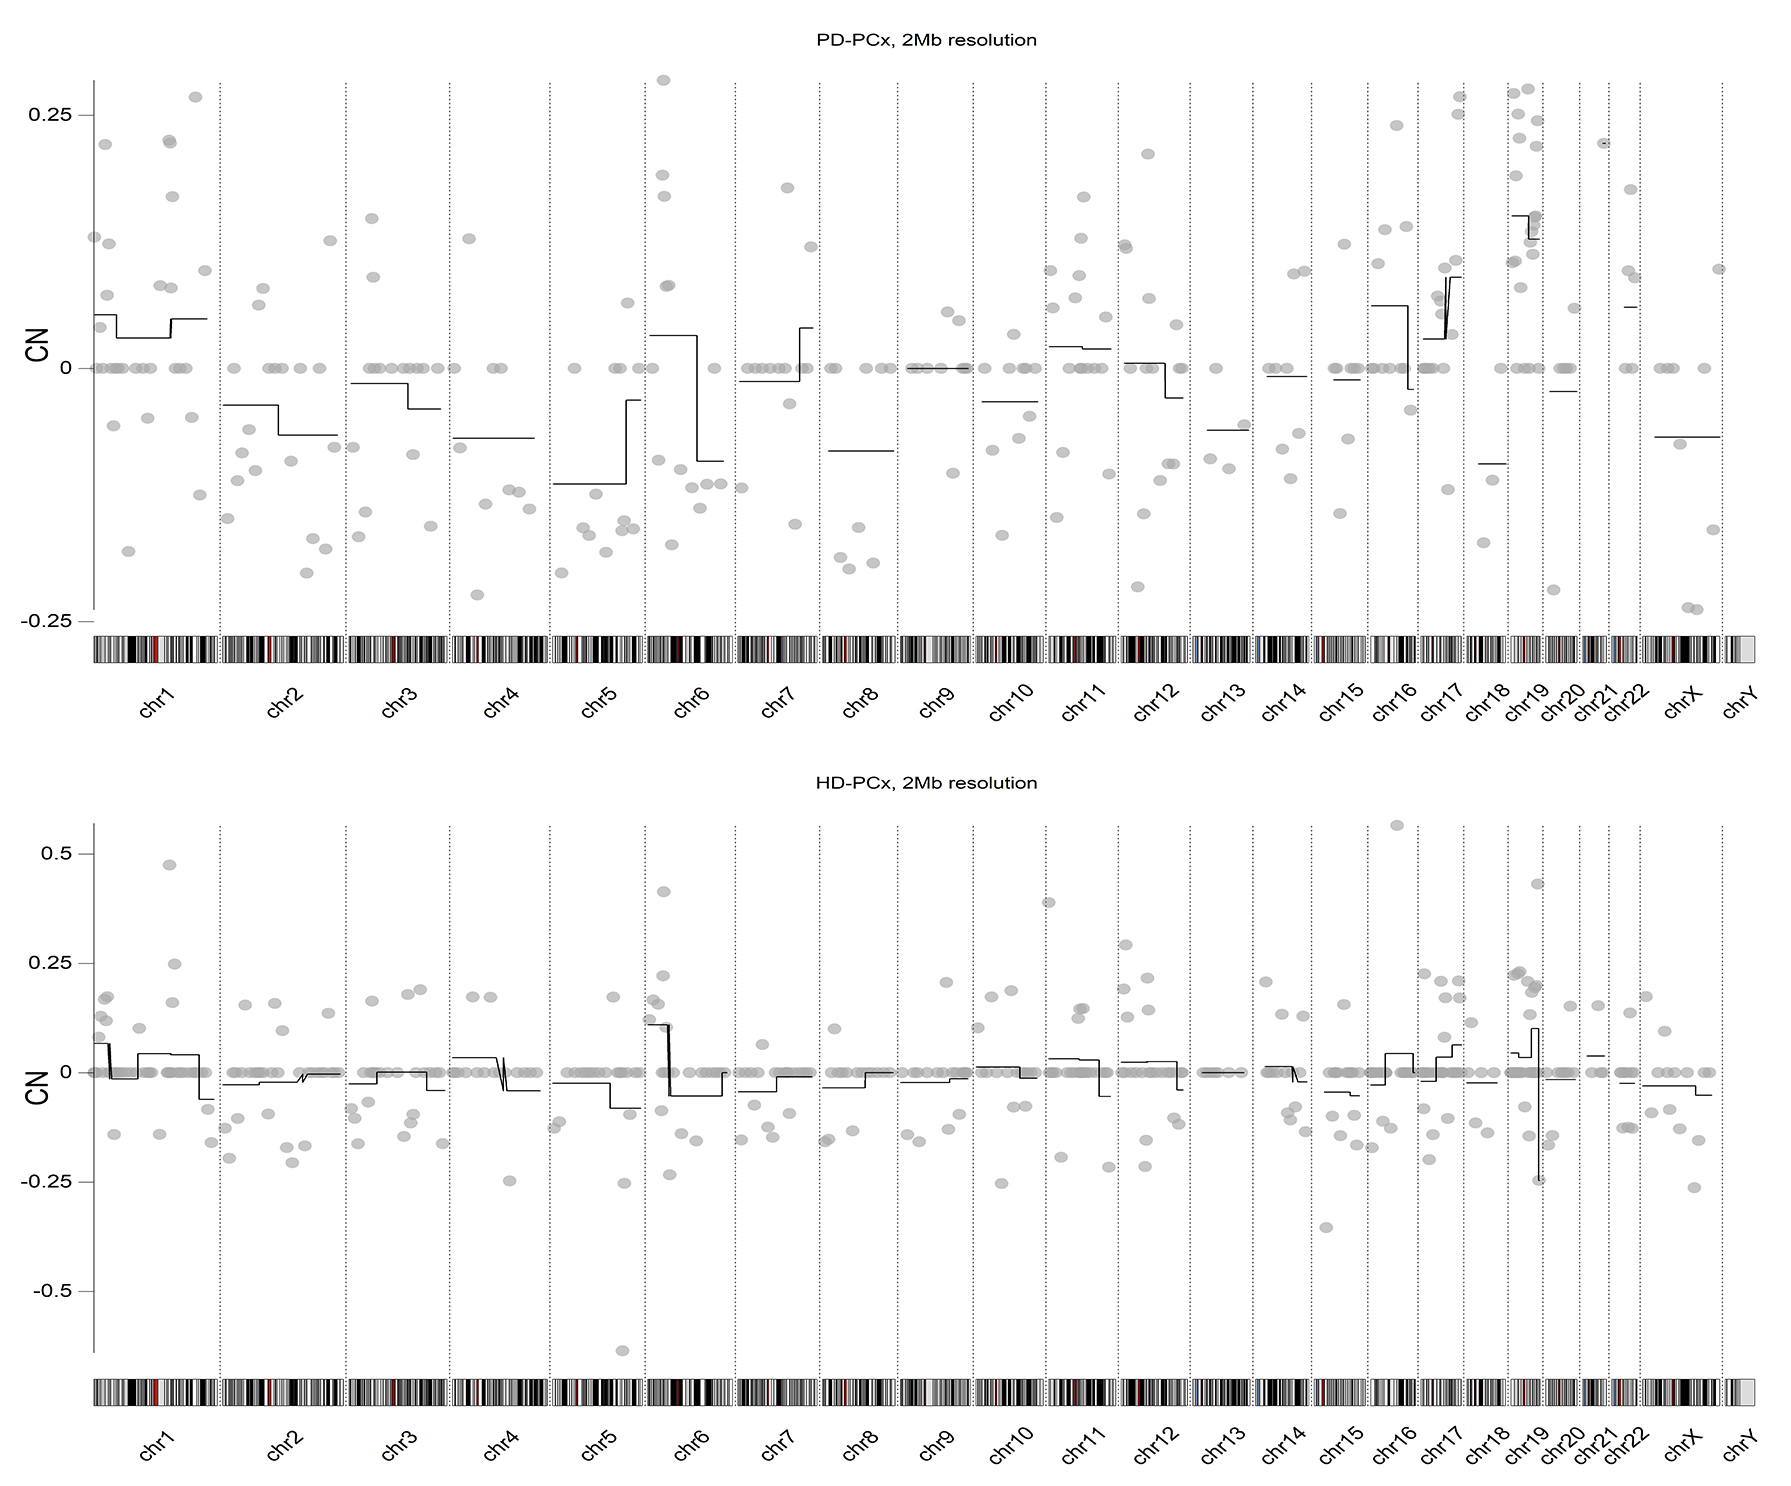
\includegraphics[width = 12.5cm]{Figures/CNV/cnv.jpg}}
\caption{Copy number variation plots for prefrontal cortex datasets.}
\label{fig:cnv-pcx}
\end{figure}

\begin{figure}[!ht] 
    \centerline{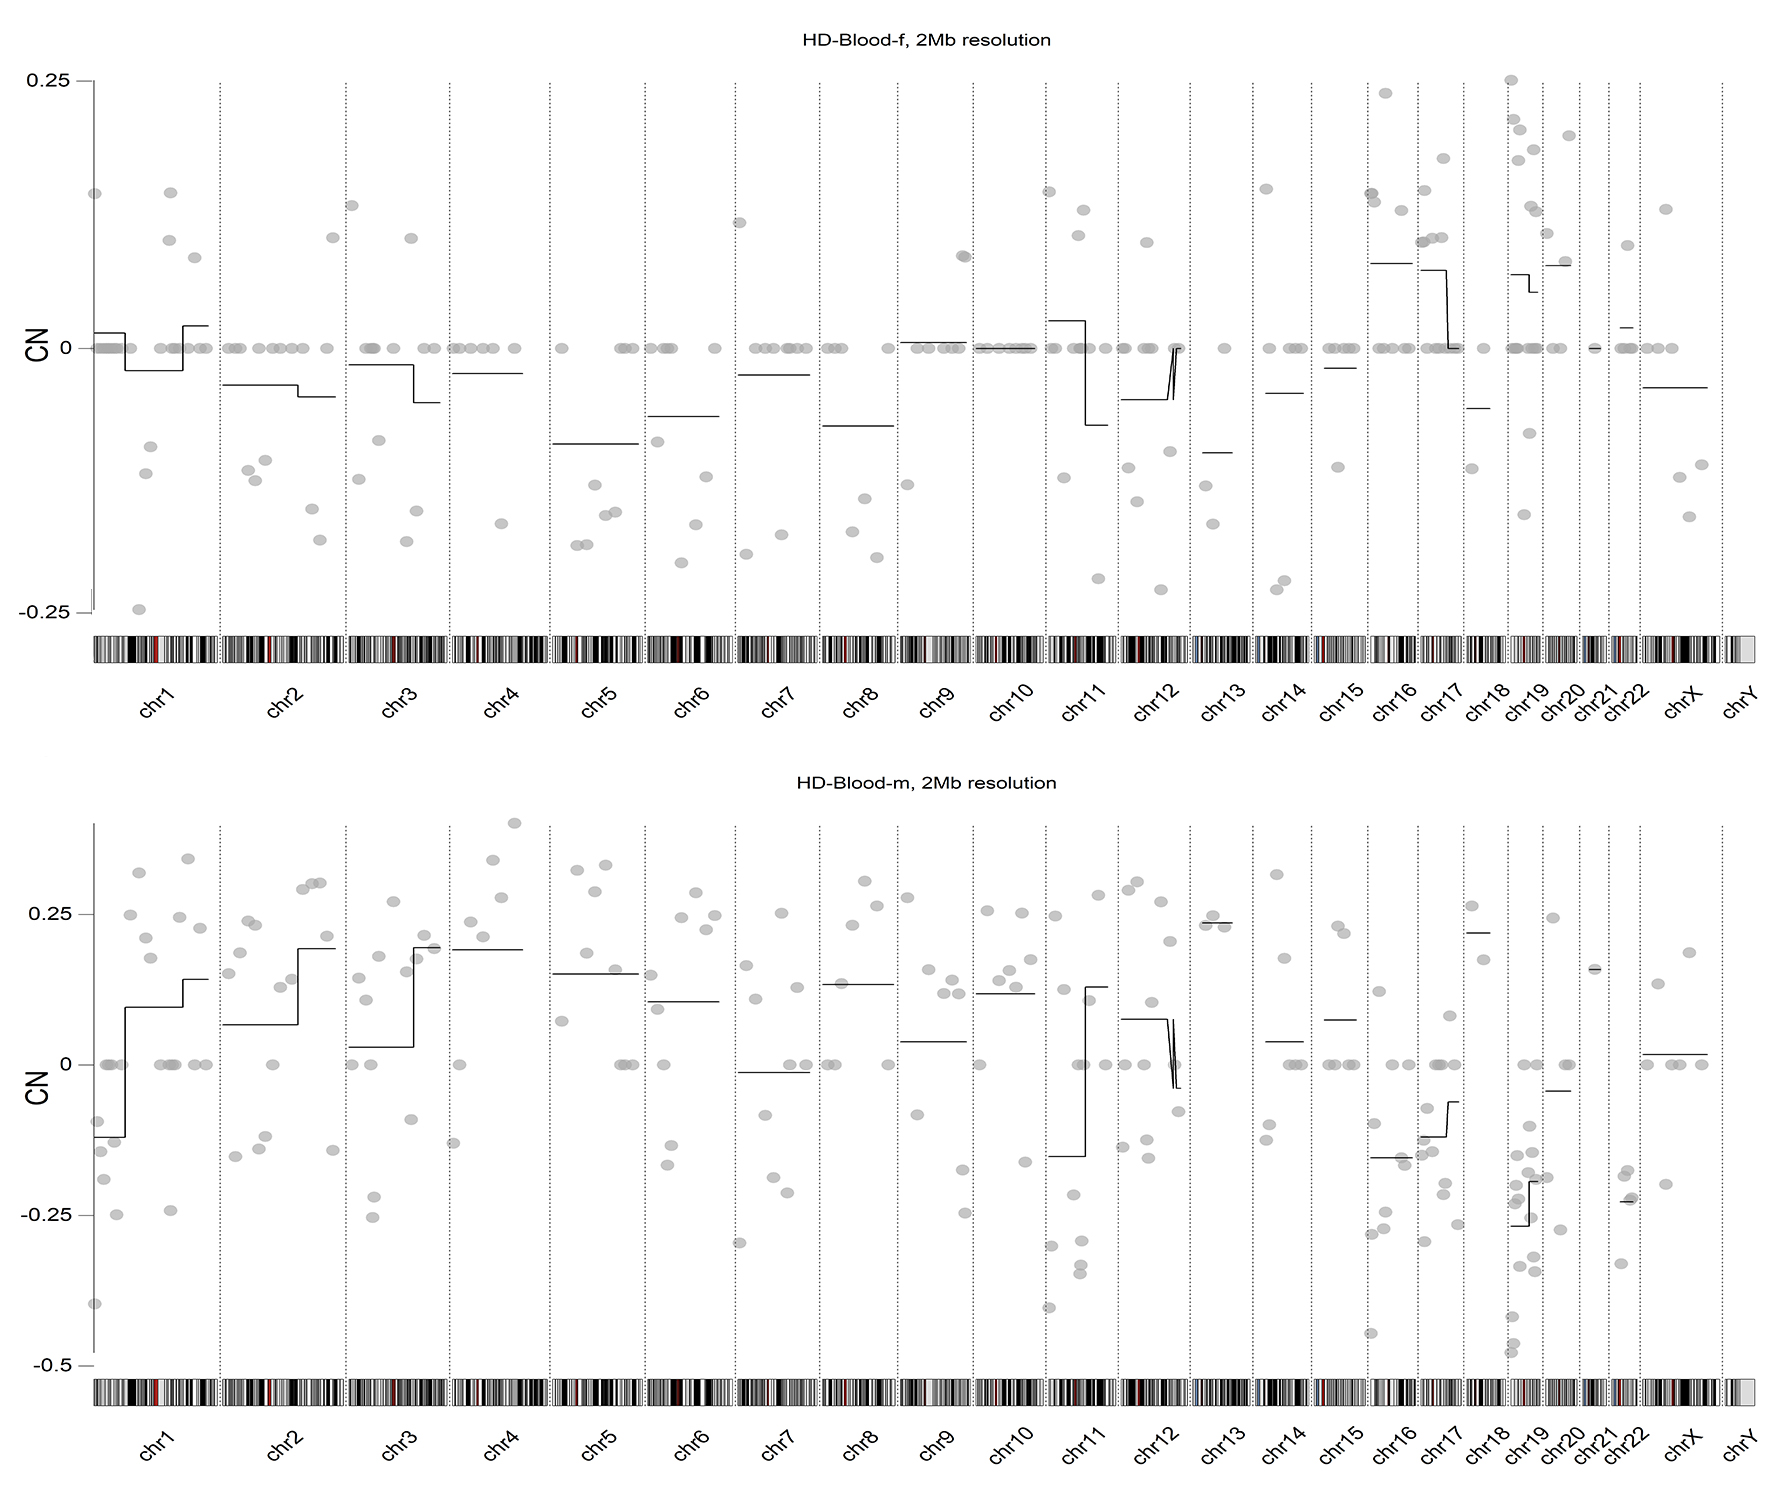
\includegraphics[width = 13cm]{Figures/CNV/cnv2.jpg}}
\caption{Copy number variation plots for Blood-HD datasets.}
\label{fig:cnv-blood}
\end{figure}

\begin{figure}[!ht] 
    \centerline{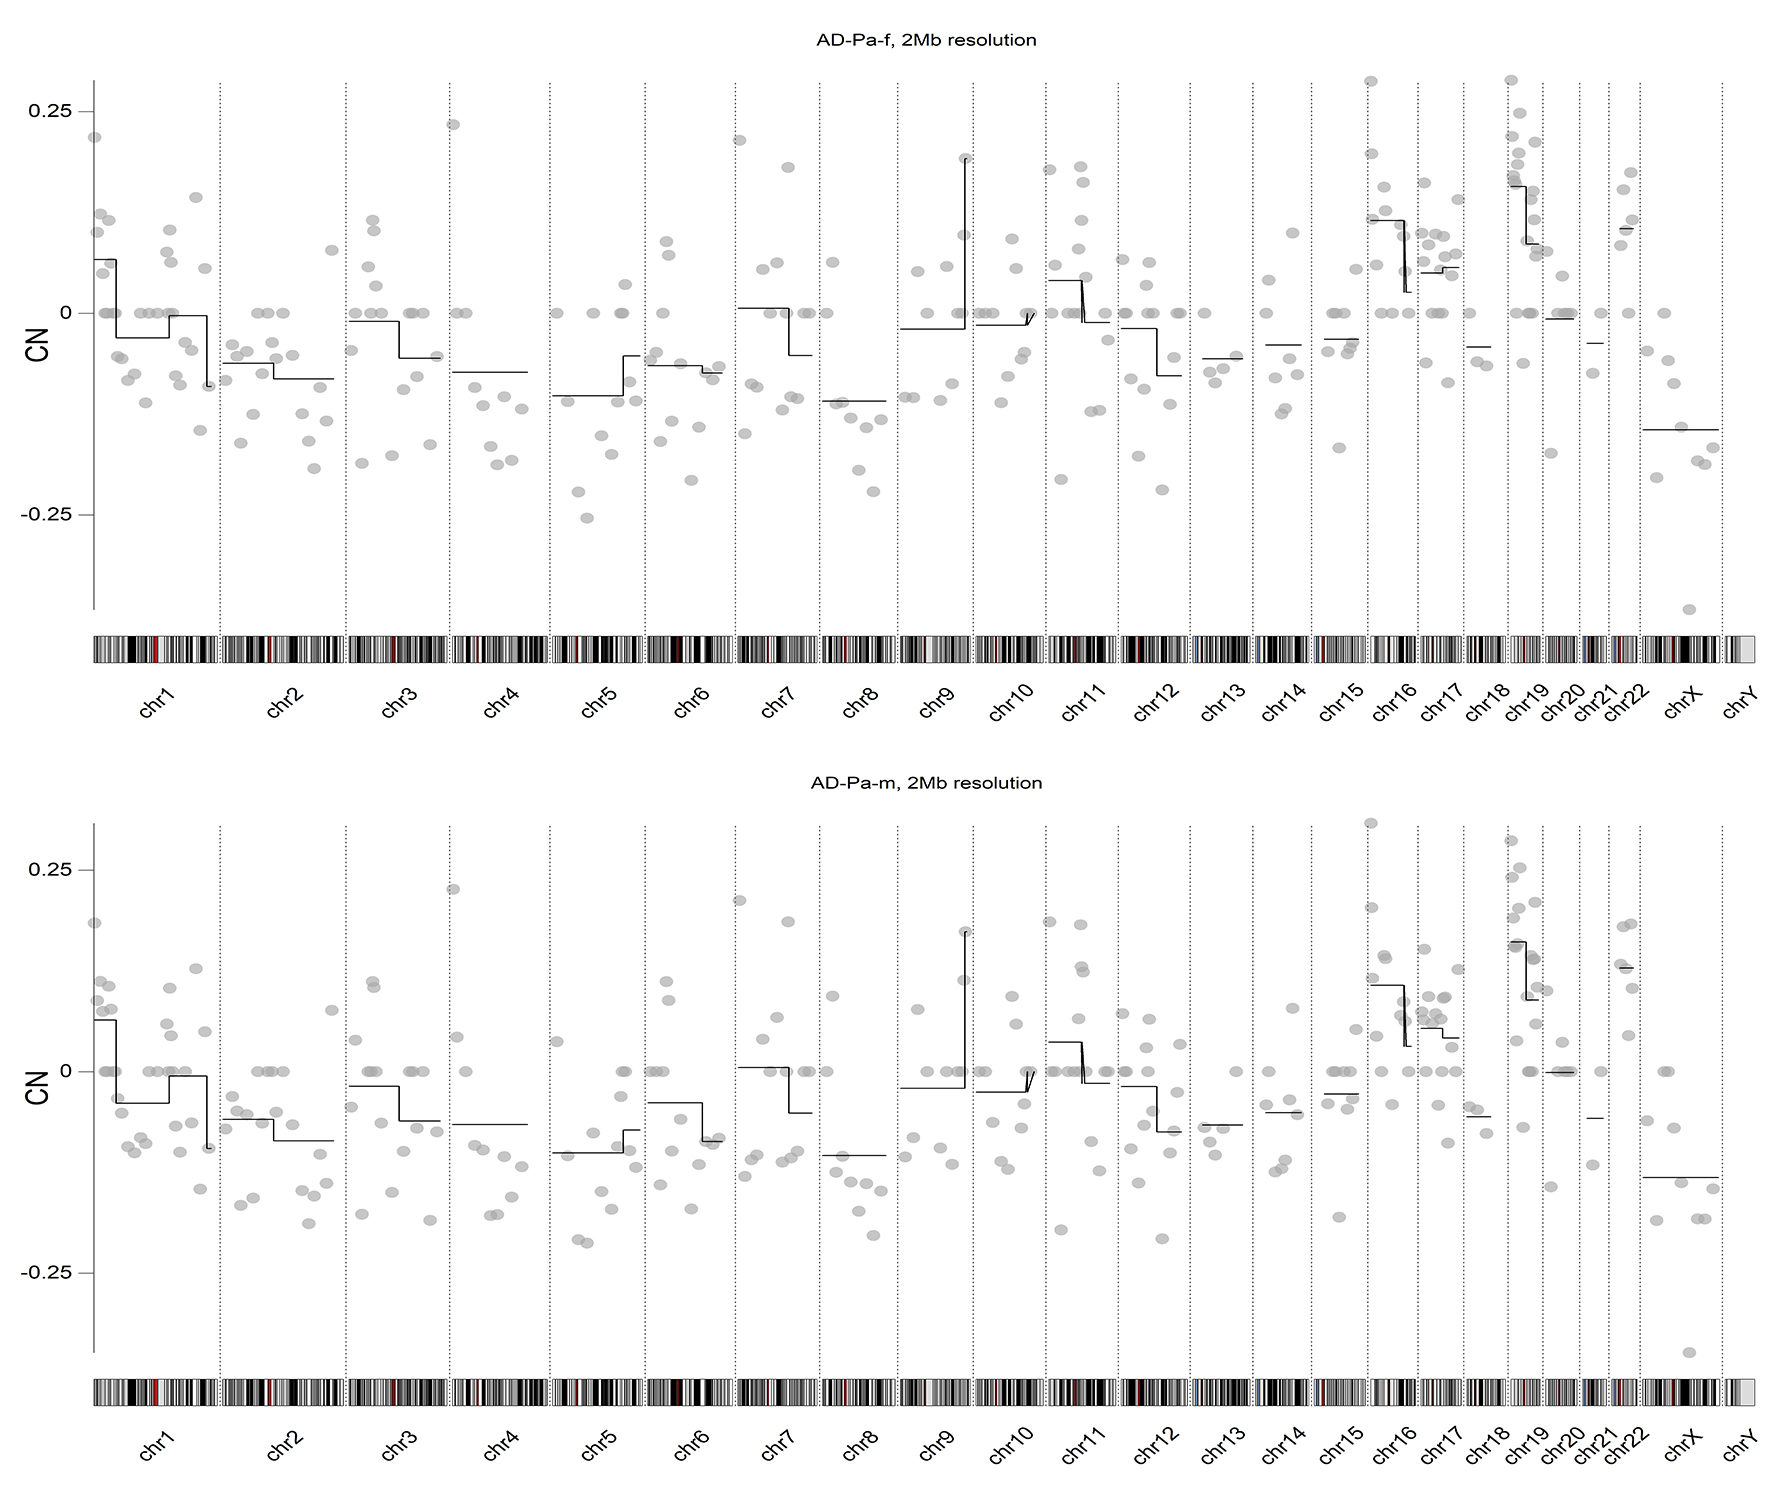
\includegraphics[width = 13cm]{Figures/CNV/cnv3.jpg}}
\caption{Copy number variation plots for Pa-AD datasets.}
\label{fig:cnv-pa}
\end{figure}

\begin{figure}[!ht] 
    \centerline{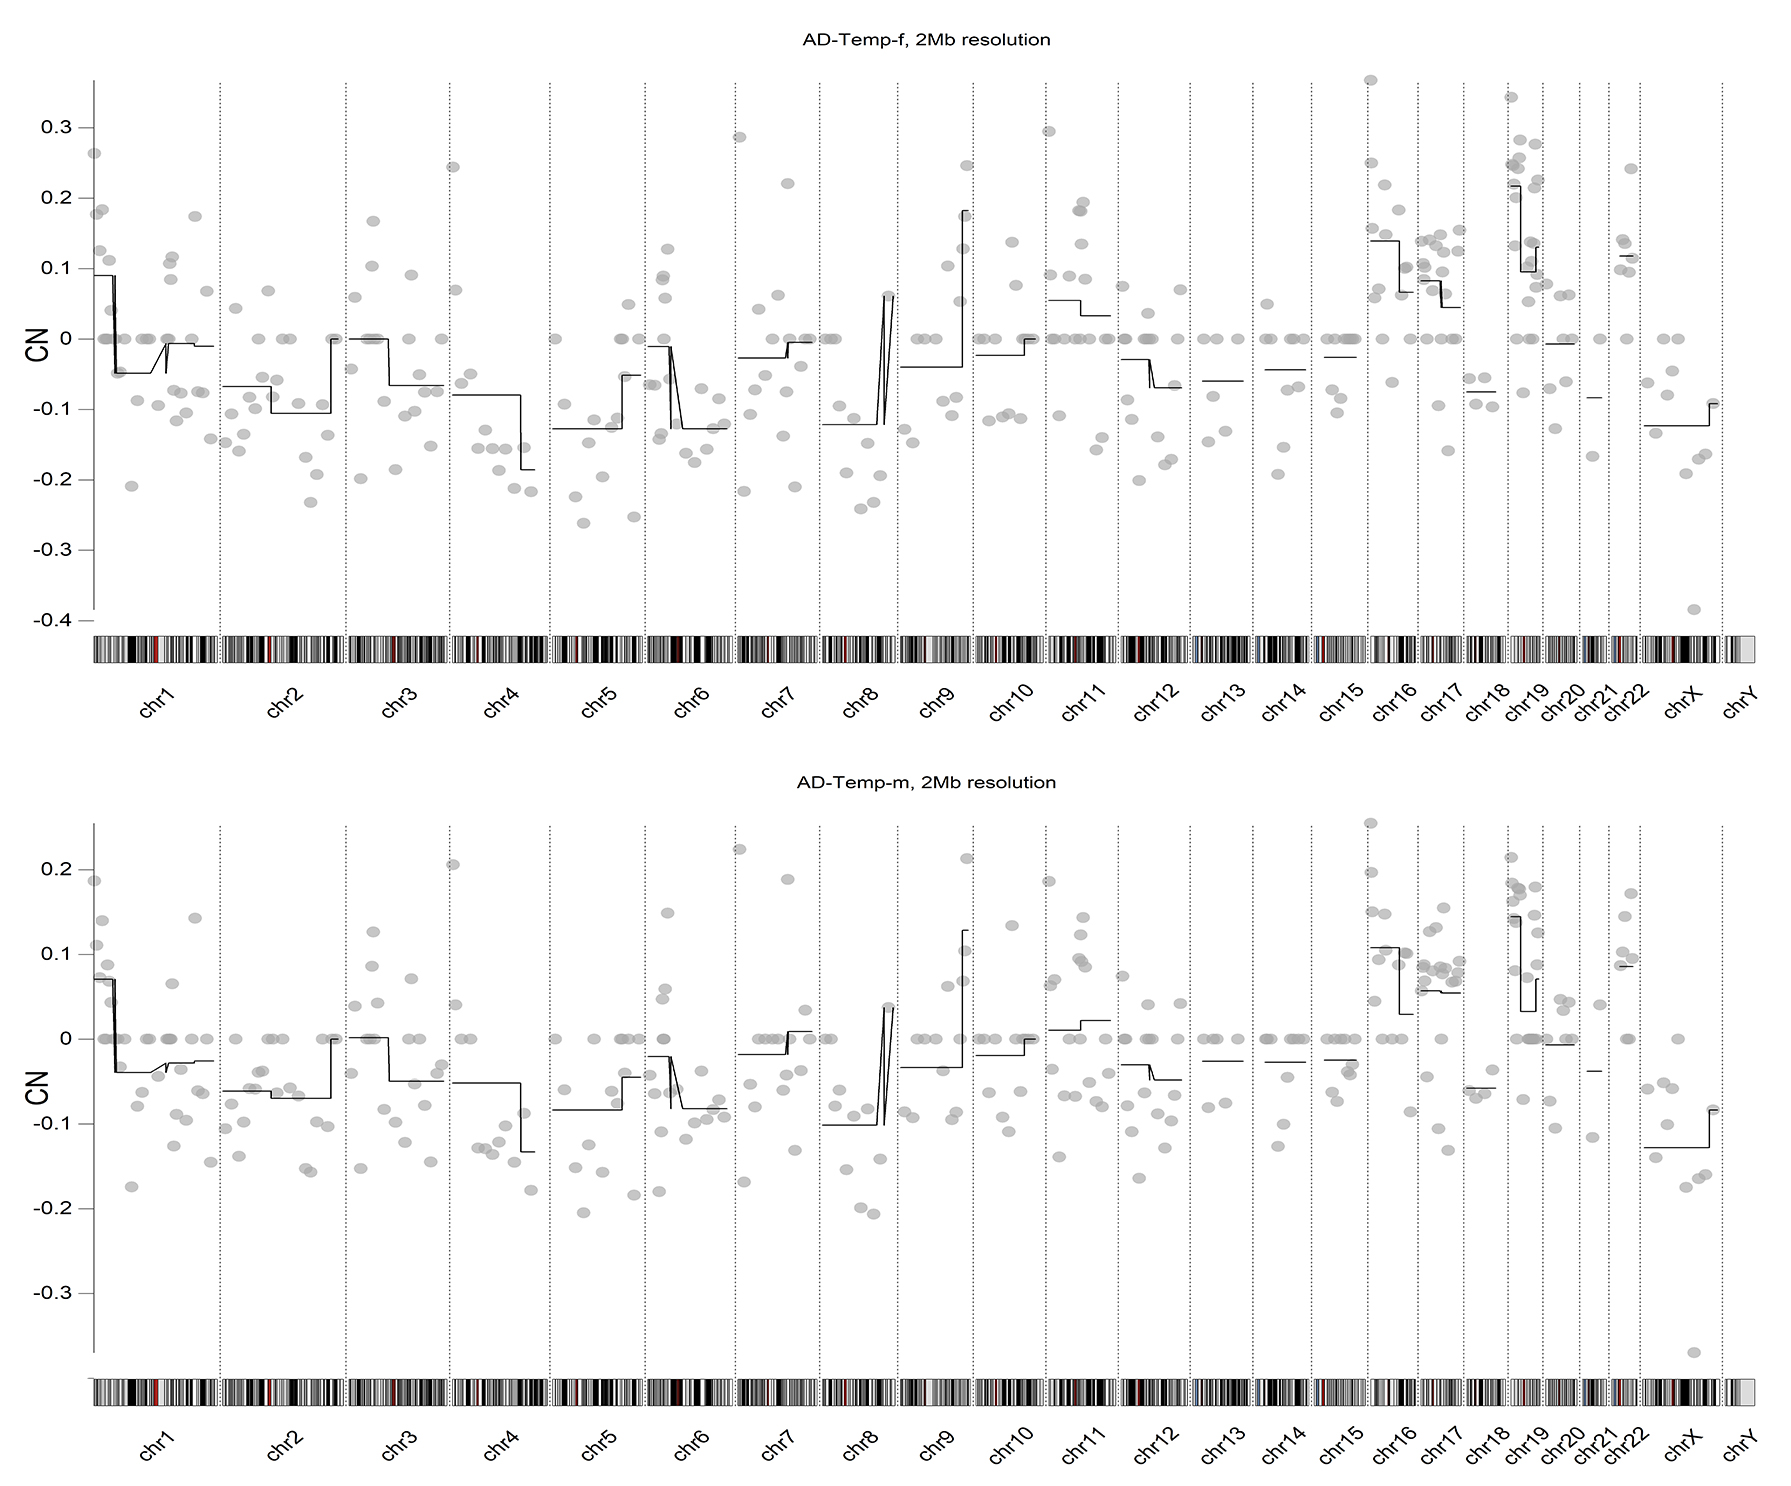
\includegraphics[width = 13cm]{Figures/CNV/cnv4.jpg}}
\caption{Copy number variation plots for Temp-AD datasets.}
\label{fig:cnv-temp}
\end{figure}

\begin{figure}[!ht] 
    \centerline{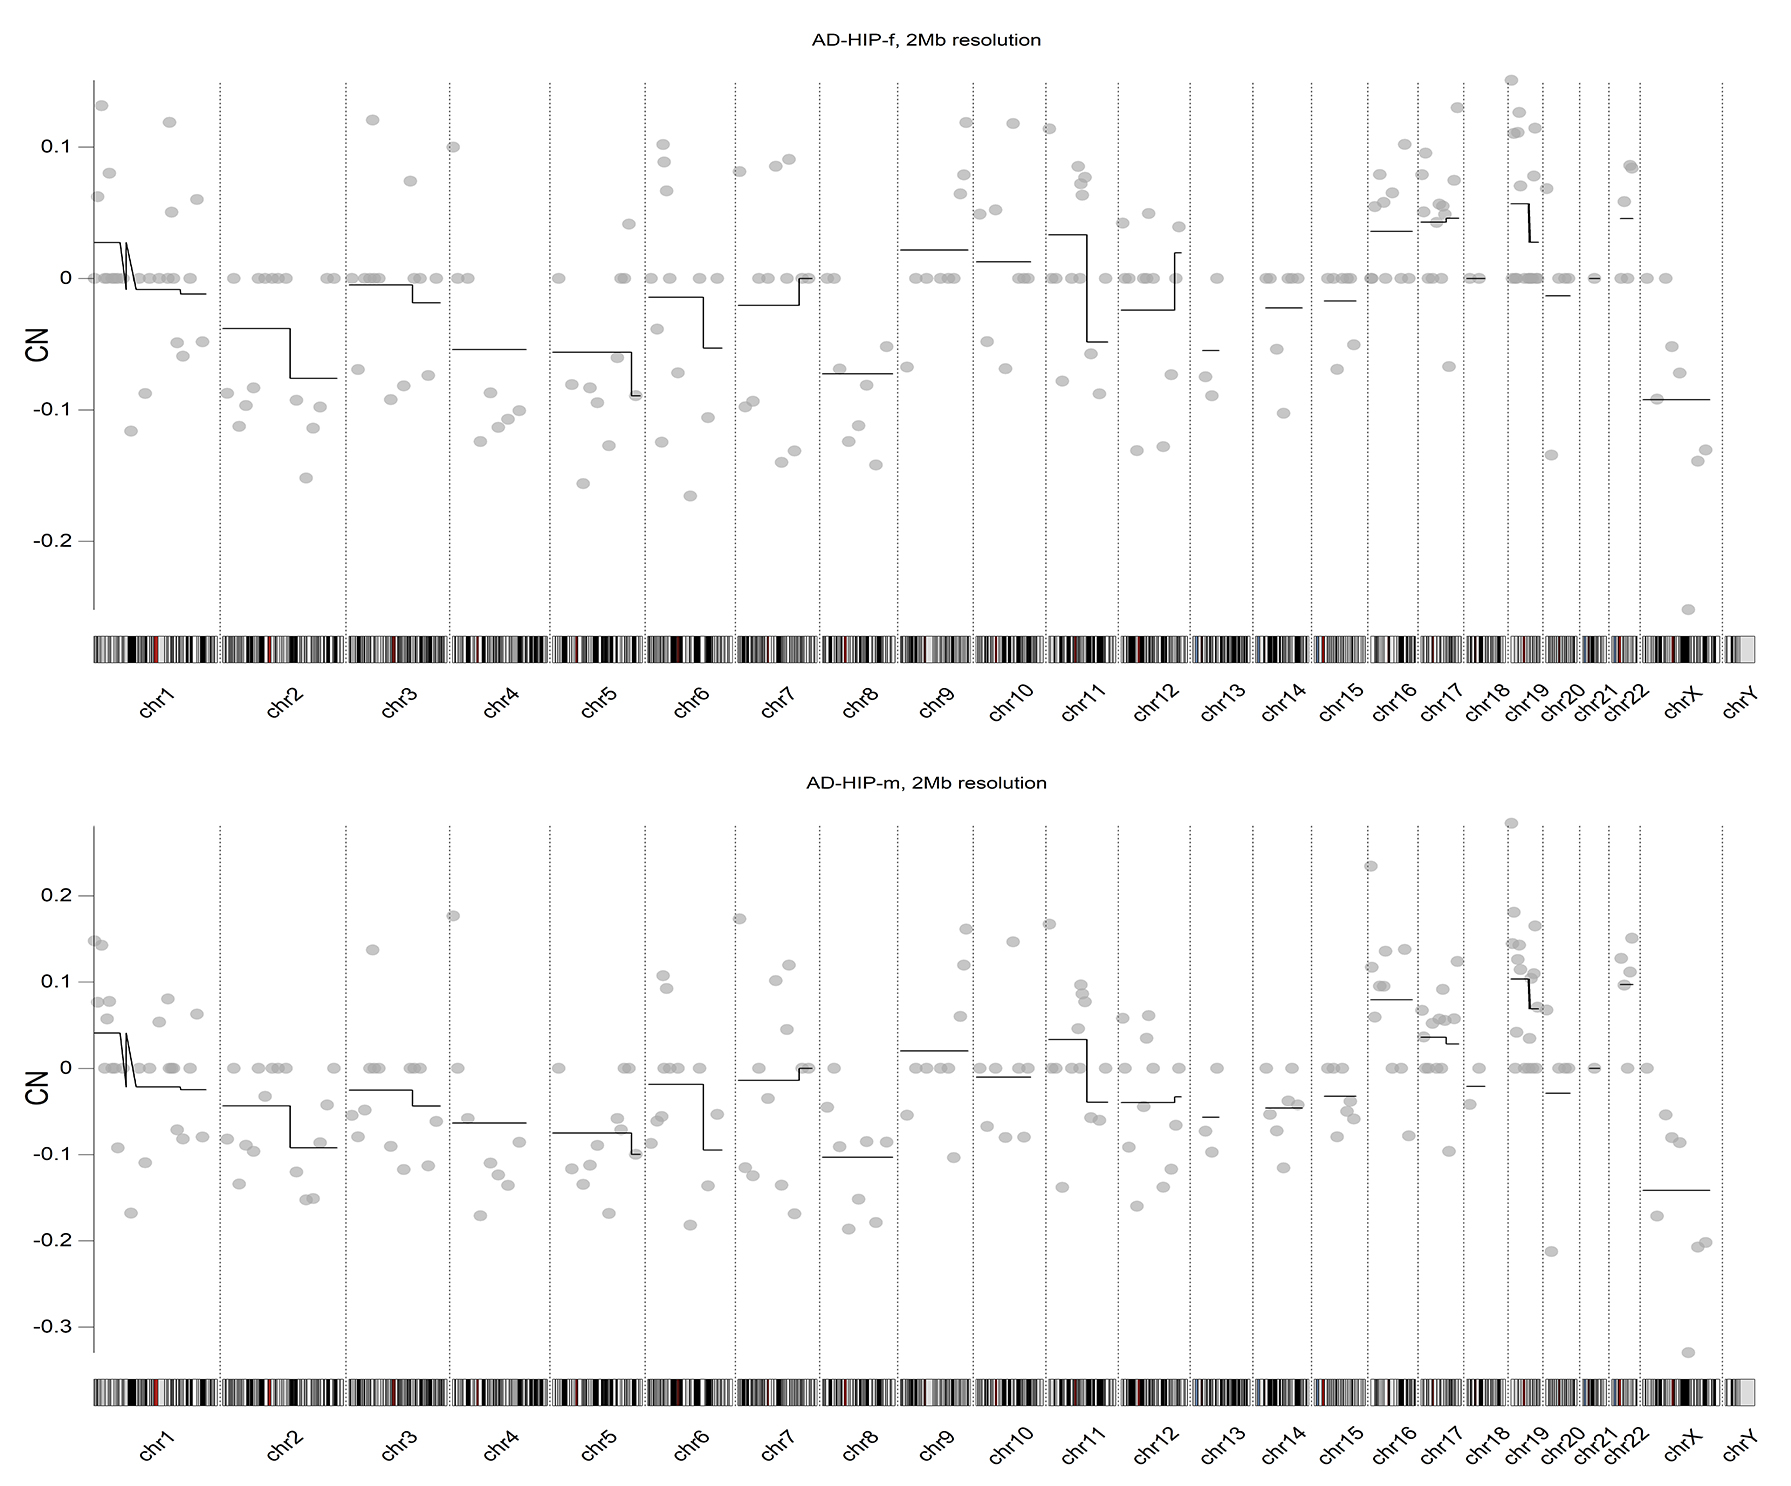
\includegraphics[width = 13cm]{Figures/CNV/cnv5.jpg}}
\caption{Copy number variation plots for Hip-AD datasets.}
\label{fig:cnv-hip}
\end{figure}

\begin{figure}[!ht] 
    \centerline{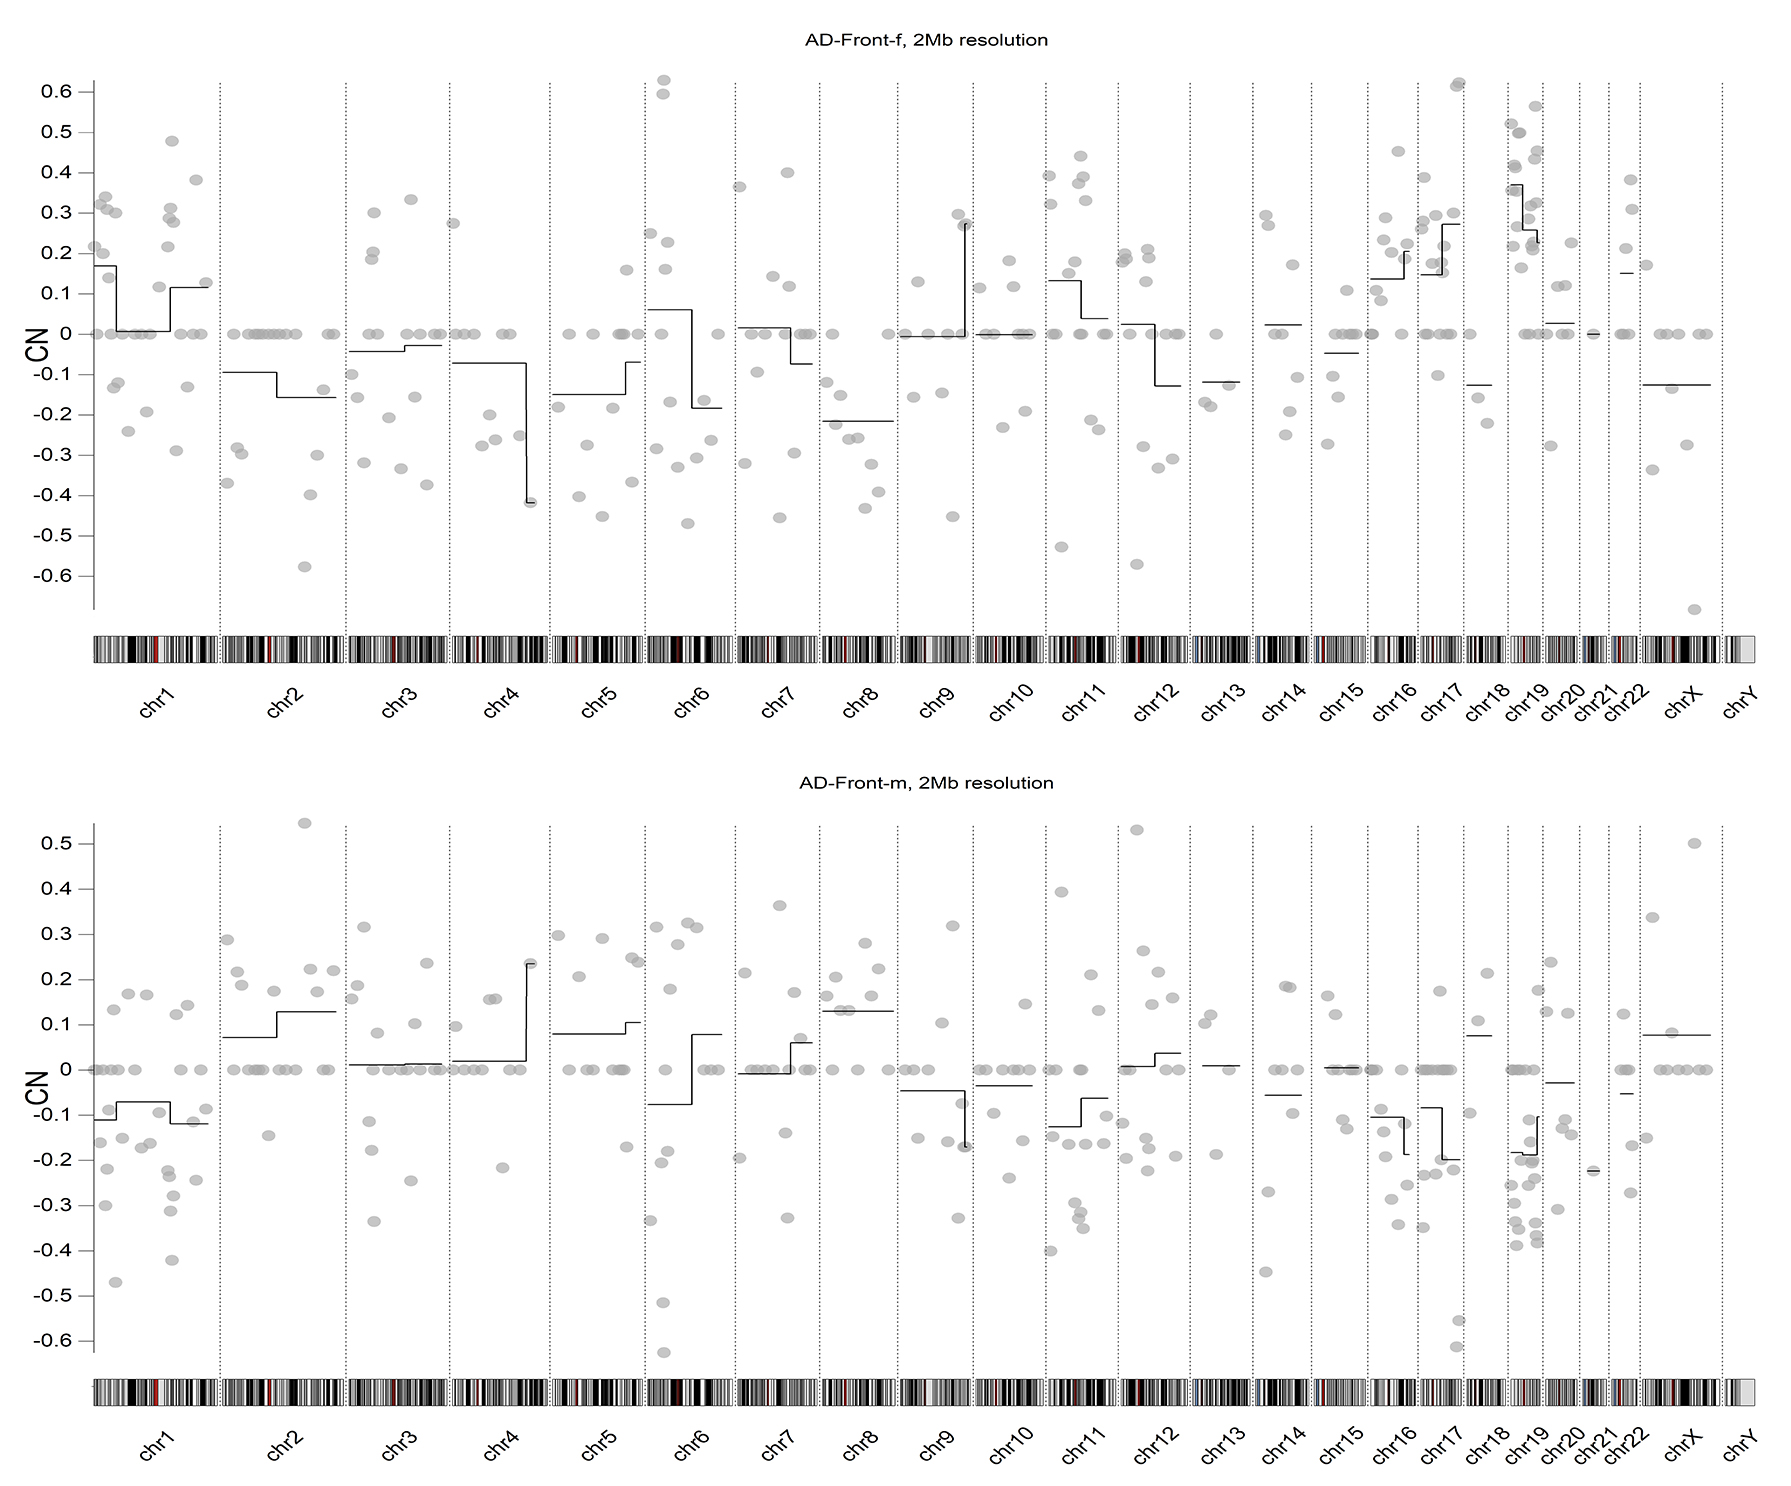
\includegraphics[width = 13cm]{Figures/CNV/cnv6.jpg}}
\caption{Copy number variation plots for Front-AD datasets.}
\label{fig:cnv-front}
\end{figure}

\begin{figure}[!ht] 
    \centerline{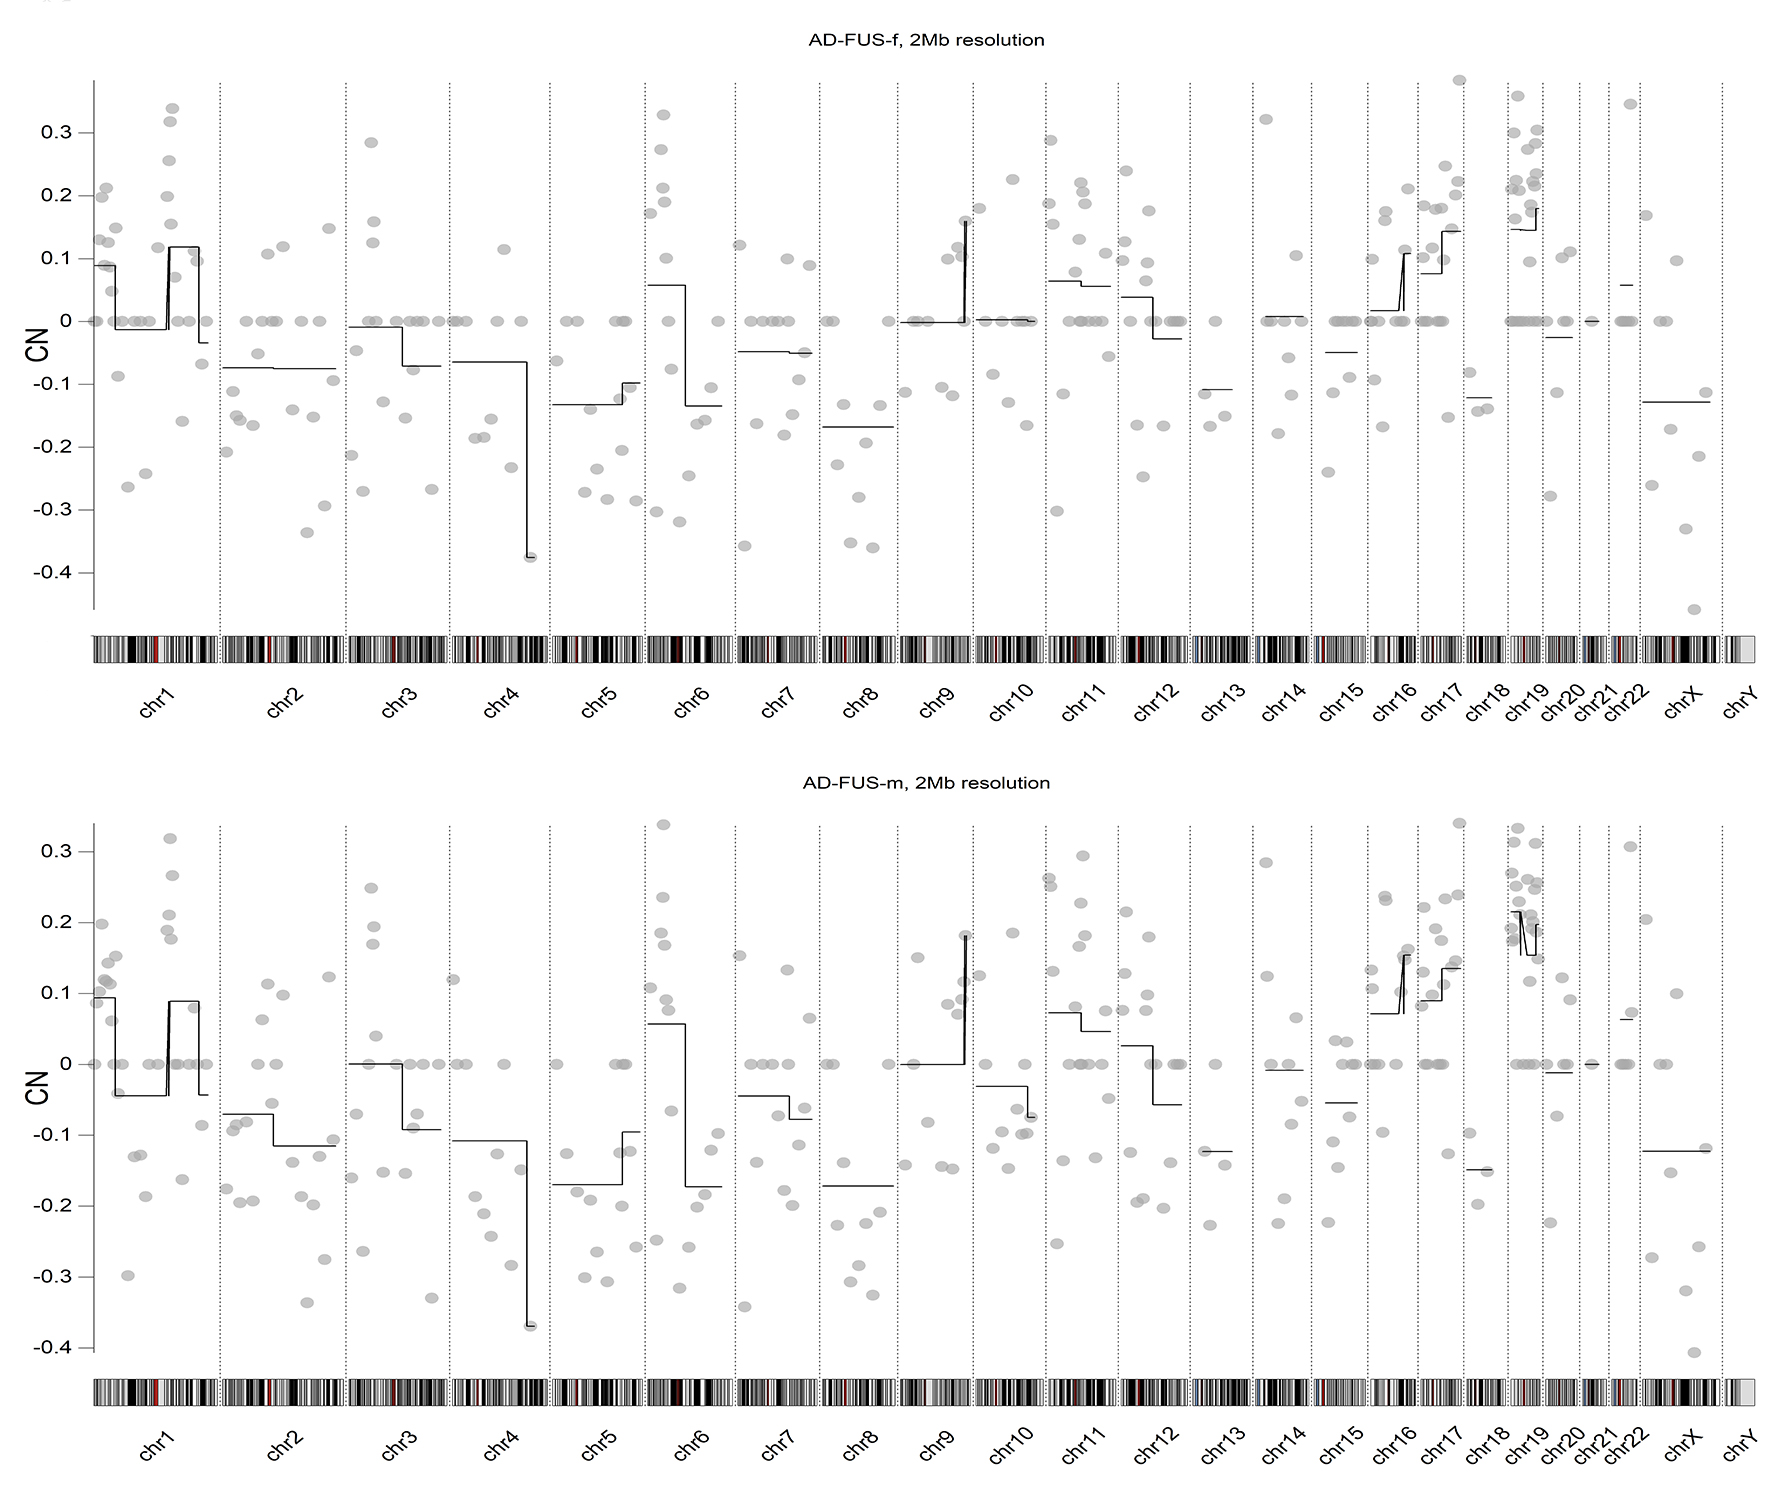
\includegraphics[width = 13cm]{Figures/CNV/cnv7.jpg}}
\caption{Copy number variation plots for Fus-AD datasets.}
\label{fig:cnv-fus}
\end{figure}
